\section{Summary}

\begin{frame}{An Opportunity for a Stupid Joke}
    \begin{block}{Henri Poincaré}
        \emph{``[L]a mathématique est l'art de donner le même nom à des choses différentes.''}
    \end{block}

\begin{figure}
\centering
\begin{minipage}{.5\textwidth}
  \centering
  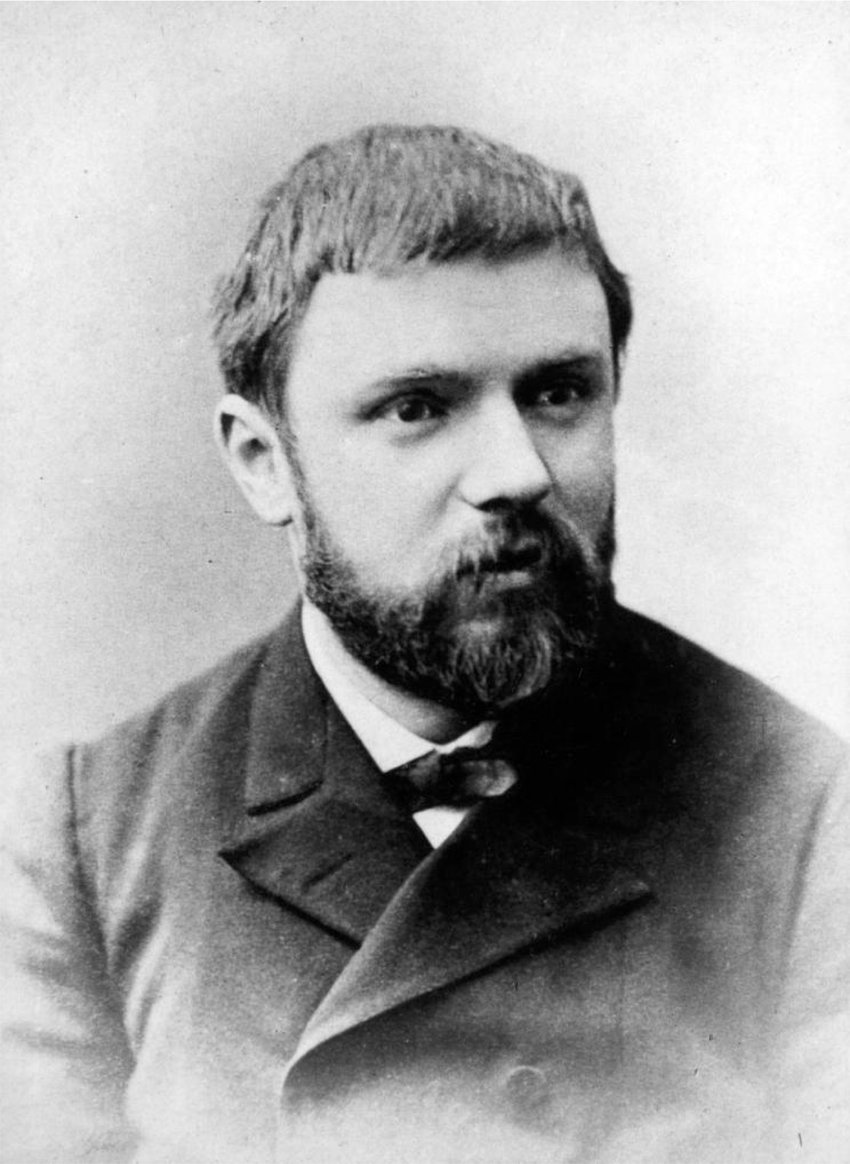
\includegraphics[width=.5\linewidth]{resources/poincare.jpg}
  \captionof{figure}{H. Poincaré, 1887.}
  \label{fig:test1}
\end{minipage}%
\begin{minipage}{.5\textwidth}
  \centering
  
\includegraphics[height=.6\linewidth]{resources/meme.jpg}
  \captionof{figure}{H. Poincaré, colourised.}
  \label{fig:test2}
\end{minipage}
\end{figure}

\end{frame}

\begin{frame}

The solution to the salmon conjecture is equivalent to:
    \begin{itemize}
        \item the mixture of four models for three independent variables;
        \item the fourth secant variety of the Segre variety $\PP^{3} \times \PP^{3} \times \PP^{3}$;
        \item the set of $(4 \times 4 \times 4)$-tables of tensor rank $\leq 4$;
        \item the naive Bayes model with four classes and three features;
        \item the conditional independence model $[ X_{1} \indep X_{2} \indep X_{3} | Y ]$;
        \item the general Markov model for the phylogenetic tree, $K_{1,3}$;
        \item superposition of four pure states in a quantum system.
    \end{itemize}

\end{frame}

\begin{frame}

    \begin{block}{A `Statistics to Algebraic Geometry' Lexicon}

    \begin{table}[]
    \begin{tabular}{lll}
    Statistics                &   & Algebra/Geometry \\ \hline
                              &   &                  \\ 
    independence              & = & Segre variety    \\ 
    exponential family        & = & toric variety    \\ 
    (log-linear models)       &   &                  \\ 
    curved exponential family & = & manifold         \\ 
    mixture model             & = & secant variety   \\
    inference                 & = & tropicalisation  \\
                              & $\vdots$ &           
    \end{tabular}
    \end{table}

    \end{block}

\end{frame}

\begin{frame}{Applications}

We finish by mentioning that algebraic statistics has at least a few important applications:

\begin{itemize}
    \item It can win you salmon;
    \item It can win you 100 Swiss francs\footnote{Not mentioned in this talk.} (CHF $100 \sim$ £$85$);
    \item One gets to learn lots of polysyllabic words;
    \item It can provide an individual with a topic for an (excellent) colloquium talk;
    \item Algebraists \& statisticians \emph{could} talk to one other (not that they \emph{would} want to).
\end{itemize}

\end{frame}